\chapter{Mathematical Foundations}
\label{ch:math}
\epigraph{By relieving the brain of all unnecessary work, a good notation sets it free to concentrate on more advanced problems, and, in effect, increases the mental power of the race.}{\textsc{Alfred North Whitehead}}
  \section{Coordinate Frames}

Before we can present the main contributions of this thesis, it will be useful to first outline the notation and mathematical foundations that underly the work. Throughout this thesis, we largely follow the notation of \cite{Barfoot2017-ri} when dealing with three-dimensional rigid-body kinematics. 

\begin{figure}[h!]
\center
\tdplotsetmaincoords{60}{110}
%
\pgfmathsetmacro{\rvec}{1.75}
\pgfmathsetmacro{\thetavec}{45}
\pgfmathsetmacro{\phivec}{60}
%
\begin{tikzpicture}[scale=5,tdplot_main_coords]
\coordinate (O) at (0,0,0) node[anchor=south east]{$\CoordinateFrame{o}$};
\draw[very thick,->, red] (0,0,0) -- (0.7,0,0);
\draw[very thick,->, green] (0,0,0) -- (0,0.7,0);
\draw[very thick,->, blue] (0,0,0) -- (0,0,0.7);
\tdplotsetcoord{V}{\rvec}{\thetavec}{\phivec}
\tdplotsetrotatedcoords{\phivec}{\thetavec}{0} 
\tdplotsetrotatedcoordsorigin{(V)}

\draw [fill, tdplot_rotated_coords] (.3,.3,.3) circle [radius=0.01] node[anchor=north west]{$p$};
\draw[-stealth,tdplot_rotated_coords, black] (O) -- (.31,.31,.31) node[midway,below] {$\VectorArrow{r}^{po}$} ;


\end{tikzpicture}
\caption{A position vector expressed in a coordinate frame.}
\end{figure}

We refer to a three-dimensional position vector, $\VectorArrow{r}^{po}$, as one that originates at the origin of a coordinate reference frame, $\CoordinateFrame{o}$, and terminates at the point $p$. This geometric quantity has the numerical coordinates $\Vector{r}^{po}_o$ when expressed in $\CoordinateFrame{o}$. Often, we will refer to two reference frames such as a world or \textit{inertial} frame,  $\CoordinateFrame{i}$, and a vehicle frame, $\CoordinateFrame{v}$. Rotation matrices or rigid-body transformations that convert coordinates from $\CoordinateFrame{i}$ to $\CoordinateFrame{v}$ will be represented as $\Transform_{vi}$, and $\Rotation_{vi}$\footnote{We use $\Rotation$ and not $\Matrix{R}$ for rotation matrices to avoid confusion with common notation for measurement model covariance.}, respectively. 


\begin{figure}[h!]
\center
\tdplotsetmaincoords{60}{110}
%
\pgfmathsetmacro{\rvec}{1.75}
\pgfmathsetmacro{\thetavec}{45}
\pgfmathsetmacro{\phivec}{60}
%
\begin{tikzpicture}[scale=5,tdplot_main_coords]
\coordinate (O) at (0,0,0) node[anchor=south east]{$\CoordinateFrame{i}$};
\draw[very thick,->, red] (0,0,0) -- (0.7,0,0);
\draw[very thick,->, green] (0,0,0) -- (0,0.7,0);
\draw[very thick,->, blue] (0,0,0) -- (0,0,0.7);
\tdplotsetcoord{V}{\rvec}{\thetavec}{\phivec}
\draw[-stealth] (O) -- (V) node[midway,above] {$\VectorArrow{t}^{vi}$} ;

\tdplotsetrotatedcoords{\phivec}{\thetavec}{0} 
\tdplotsetrotatedcoordsorigin{(V)}


%Coordinate frame with label
\draw[very thick,tdplot_rotated_coords,->, red] (0,0,0) -- (.4,0,0);
\draw[very thick,tdplot_rotated_coords,->, green] (0,0,0) -- (0,.4,0);
\draw[very thick,tdplot_rotated_coords,->, blue] (0,0,0)-- (0,0,.4);
\draw[tdplot_rotated_coords] (0,0,0) node[anchor=south east] {$\CoordinateFrame{v}$};

%Local vector
\draw [fill, tdplot_rotated_coords] (.31,.31,.31) circle [radius=0.01] node[anchor=north west]{$p$};
\draw[-stealth,tdplot_rotated_coords, purple] (0,0,0) -- (.3,.3,.3) node[midway,above] {\footnotesize $\VectorArrow{r}^{pv}$};
\draw[-stealth,tdplot_rotated_coords, black] (O) -- (.3,.3,.3) node[midway,below] {$\VectorArrow{r}^{pi}$} ;

\end{tikzpicture}
\label{fig:math_two_ref_frames}
\caption{Two common references frames used throughout this thesis.}
\end{figure}



\section{Rotations} 

The rotation matrix $\Rotation$ is a member of the matrix Lie group $\LieGroupSO{3}$ (the Special Orthogonal group),
\begin{equation}
\LieGroupSO{3} = \{ \Rotation \in \Real{}^{3 \times 3} | ~ \Rotation^T\Rotation = \Matrix{1}, \det{\Rotation} = 1  \}.	
\end{equation}
\subsubsection{Active vs. Passive}
An active (or \textit{alibi}) rotation changes the coordinates of a position directly while implicitly assuming that the reference frame is fixed. A passive (or \textit{alias}) rotation rotates the reference frame. Following \cite{Barfoot2017-ri}, all rotation matrices in this dissertation are passive unless otherwise noted.  

\subsubsection{Exponential and Logarithmic Maps}

Since rotations form a matrix Lie group (we refer the reader to \cite{Sola2018-kg} and \cite{Barfoot2017-ri} for a thorough treatment of Lie groups for state estimation), we can define a surjective exponential map\footnote{We follow \cite{Sola2018-kg} and also define \textit{capitalized} map for notational clarity.} from three axis-angle parameters, $\RotationVector = \phi \RotationAxisVector, ~~ \phi \in \Real{}, \RotationAxisVector \in S^2$, to a rotation matrix, $\Rotation$: 
\begin{align}
\label{eq:so3_exp}
\Rotation = \MatExp{\Vector{\phi}} = \Matexp{\Vector{\phi}} &= \sum_{n=0}^{\infty}  \frac{1}{n!} {(\Vector{\phi}^\wedge)}^n\\
\label{eq:euler_rodriguez}
&= \cos{\phi} \IdentityMatrix + (1 - \cos{\phi}) \RotationAxisVector\RotationAxisVector^T + \sin{\phi} \RotationAxisVector^\wedge,
\end{align}
where the wedge operator $(\cdot)^\wedge$\footnote{This operator is sometimes also expressed as $(\cdot)^\times$ or $[\cdot]_\times$ and is known as the skew-symmetric operator.} is defined as
\begin{equation}
\RotationAxisVector^\wedge = \bbm a_0 \\ a_1 \\ a_2 \ebm^\wedge = \bbm 0 & -a_2 & a_1 \\ a_2 & 0 & -a_0 \\ -a_1 & a_0 & 0 \ebm.	
\end{equation}
\Cref{eq:euler_rodriguez} is often referred to as the Euler-Rodriguez formula and it can also be derived geometrically, starting from Euler's theorem that any rotation can be expressed as an axis of rotation and an angle of rotation about that axis. Although  the map in \Cref{eq:so3_exp} is surjective, we can define an inverse map if we restrict its domain to $0 \leq \phi < \pi$:
\begin{align}
\label{eq:so3_log}
\RotationVector =  \MatLog{\Rotation} = \Matlog{\Rotation} &= \frac{\phi (\Rotation - \Rotation^T)^\vee}{2 \sin{\phi}}, 
\end{align}
where $\phi = \arccos{\left(\frac{\Trace{\Rotation} - 1}{2}\right)}$ and the \textit{vee} operator, $(\cdot)^\vee : \Real{}^{3 \times 3} \rightarrow \Real{}^3$, is defined as the unique inverse of the wedge operator $(\cdot)^\wedge$. Note \Cref{eq:so3_log} is undefined at both $\phi = 0$ and at $\phi = \pi$. In the former case, we can use a small-angle approximation and define

\begin{equation}
	\MatLog{\Rotation} \approx (\Rotation - \IdentityMatrix)^\vee ~~ \textrm{when} ~~ \phi \approx 0. 
\end{equation}

The latter case (when $\phi = \pi$) defines the \textit{cut locus} of the space where $\MatExp{\cdot}$ is not a covering map and both $+\RotationVector$ and $-\RotationVector$ map to the same $\Rotation$. This \textit{cut locus} is related to the idea that any three parameterization of $\LieGroupSO{3}$ will have singularities associated with it.

\subsection{Unit Quaternions}

Another way (and historically, the original way) to represent a general rotation is to use a unit quaternion, $\quat$. A unit quaternion consists of a scalar value $q_\omega$, and a three-dimensional vector component, $\quat_v$:
\begin{equation}
	\quat = \bbm q_\omega \\ \quat_v \ebm \in S^3, ~~ (\Norm{\quat} = 1).
\end{equation}

Unit quaternions also form a Lie group \citep{Sola2018-kg} and and lie on a three-dimensional unit sphere within $\Real{}^4$. This manifold represents a double cover of $\LieGroupSO{3}$ (since both $\quat$ and $-\quat$ represent the same rotation)\footnote{$\LieGroupSO{3}$ is diffeomorphic to RP(3) (the real projective space) which can be made by `identifying' antipodal points in $S^3$ (unit sphere in $\RealNumbers^4$). Since unit quaternions belong to $S^3$, they represent a double cover of $\LieGroupSO{3}$ since we have not identified $\quat$ and $-\quat$.}. As with rotation matrices, we can define a surjective map from three parameters to the group itself,

\begin{equation}
\quat = \MatExp{\RotationVector} = \bbm \cos{(\phi/2)} \\ \RotationAxisVector \sin{(\phi/2)} \ebm.	
\end{equation}
Similarly, we can also define a logarithmic map as
\begin{align}
\label{eq:math_quat_log}
	\RotationVector =  \MatLog{\quat} = 2 \quat_v \frac{\arctan{(\Norm{\quat_v},  q_\omega})}{\Norm{\quat_v}}.
\end{align}

\noindent To avoid issues with the double cover, we replace $\quat$ with $-\quat$ if $q_\omega$ is negative before evaluating \Cref{eq:math_quat_log}. Also note again that \Cref{eq:math_quat_log} is undefined when $\phi = 0$, but, importantly, we do not face any issues when $\phi = \pi$ due to the half-angle. As with rotation matrices, we can use small angle approximations to define:

\begin{equation}
	\MatLog{\quat} \approx \frac{\quat_v}{q_\omega} \left( 1 - \frac{\Norm{\quat_v}^2}{3 q_\omega^2}\right) ~~ \textrm{when} ~~ \phi \approx 0. 
\end{equation}

A fantastic summary of the history of rotation parameterizations, unit quaternions and the story of Hamilton and Rodriguez can be found in \cite{Altmann1989-ru}.



\section{Spatial Transforms}
The rigid body transform $\Transform$ is a also a member of the matrix Lie group, the Special Euclidian group $\LieGroupSE{3}$ and can be defined as a $4 \times 4$ matrix as follows:

\begin{equation}
\LieGroupSE{3} = \{ \Transform = \bbm \Rotation & \Vector{t} \\ \Vector{0}^T & 1 \ebm \in \Real{}^{4 \times 4} | ~  \Rotation \in \LieGroupSO{3},  \Vector{t} \in \Real{}^3  \}.
\end{equation}

As a member of a matrix Lie group, it also admits a surjective exponential map,

\begin{equation}
\Transform = \MatExp{\Vector{\xi}} = \Matexp{\Vector{\xi}} = \sum_{n=0}^{\infty}  \frac{1}{n!} {(\Vector{\xi}^\wedge)}^n	
\end{equation}
where $\TransformVector = \bbm \Vector \rho \\ \Vector \phi \ebm \in \Real{}^6$ and the wedge operator is overloaded (following \cite{Barfoot2017-ri}) as follows:
\begin{equation}
  \Vector \xi^\wedge \triangleq \bbm \Vector \rho \\ \Vector \phi \ebm ^\wedge = \bbm
  \Vector \phi^\wedge & \Vector \rho \\ \Transpose{\Vector{0}} &  0 \ebm.	
\end{equation}
In practice, we can evaluate the exponential map through the Euler-Rodriguez formula (\Cref{eq:euler_rodriguez}) and by computing the left-Jacobian of $\LieGroupSO{3}$,  $\LeftJacobianSO$, 

\begin{equation}
\Transform = \MatExp{\bbm \Vector \rho \\ \Vector \phi \ebm} = \bbm \Rotation(\RotationVector) & \LeftJacobianSO(\RotationVector) \Vector{\rho} \\ \Vector{0}^T & 1 \ebm,
\end{equation}
where
\begin{equation}
\LeftJacobianSO(\RotationVector) = \frac{\sin{\phi}}{\phi} \IdentityMatrix + (1 - \frac{\sin{\phi}}{\phi}) \RotationAxisVector\RotationAxisVector^T + \frac{1 - \cos{\phi}}{\phi} \RotationAxisVector^\wedge.
\end{equation}




\subsection{Applying Transforms}
Applying our notation for coordinate frames (and referring back to \Cref{fig:math_two_ref_frames}), a transform, $\Transform_{vi}$ can be expressed as 
\begin{equation}
\Transform_{vi} = \bbm \Rotation_{vi} & \Vector{t}_v^{iv} \\ \Vector{0}^T & 1 \ebm.
\end{equation}
This allows us to use the homogenous point representation for $\Vector{r}^{pi}_i$ and express the following relation:
\begin{equation}
	\boldsymbol{r}^{pi}_v = \Transform_{vi} \boldsymbol{r}^{pi}_i,
\end{equation}
or
\begin{equation}
	\bbm \Vector{r}^{pi}_v \\ 1 \ebm = \underbrace{\bbm \Rotation_{vi} & \Vector{t}_v^{iv} \\ \Vector{0}^T & 1 \ebm}_{\Transform_{vi}} \bbm \Vector{r}^{pi}_i \\ 1 \ebm,
\end{equation}
which is numerically equivalent to  
\begin{equation}
 \Vector{r}^{pi}_v =  \Rotation_{vi} \Vector{r}^{pi}_i + \Vector{t}_v^{iv}.  
 \end{equation}

\section{Perturbations}

When solving optimization problems that involve rotations or rigid-body transforms, it is often useful to consider a small \textit{perturbation} about an operating point. By leveraging a core property of Lie groups (that they are locally `Euclidian'), we can convert difficult non-linear problems into ones that have local linear approximations.

Using rotations as an example, we can perturb an operating point, $\Mean{\Rotation} \definedtobe \MatExp{\Mean{\RotationVector}}$, in three different ways:
\begin{align}
\Rotation &= \left\{  	\begin{array}{ll}
		\MatExp{\delta \RotationVector^\ell} \Mean{\Rotation}   & \mbox{left perturbation,} \\
		\MatExp{\Mean{\RotationVector} + \delta \RotationVector^m}  & \mbox{middle perturbation,} \\
		\Mean{\Rotation} ~ \MatExp{\delta \RotationVector^r}  & \mbox{right perturbation.}  \\
	\end{array}
	\right.
\end{align}
We can relate all the left and middle perturbations through the left Jacobian of $\LieGroupSO{3}$ with the following useful identity,
\begin{equation}
\MatExp{( \RotationVector + \delta \RotationVector^m)} \approx \MatExp{\LeftJacobianSO(\RotationVector) \delta \RotationVector^m} \MatExp{\RotationVector}.	
\end{equation}
From this it follows that $\delta \RotationVector^\ell \approx \LeftJacobianSO(\RotationVector) \delta \RotationVector^m$ and elucidates why $\LeftJacobianSO$ is called the \textit{left} Jacobian. 

In this dissertation, we will use the left and middle perturbations when appropriate. Using small angle approximations, the Euler-Rodriguez formula (\Cref{eq:euler_rodriguez}) yields $\MatExp{\delta \RotationVector} \approx \IdentityMatrix + \delta \RotationVector^\wedge$, which allows us to write the useful formula for the left perturbation:
\begin{equation}
	\Rotation = (\IdentityMatrix + (\delta \RotationVector^\ell)^\wedge) \Mean{\Rotation}.
\end{equation}
Similarly, we can write analogous expressions for a rigid body transform, $\Transform \in \LieGroupSE{3}$, as composed of an operating point $\Mean{\Transform} \definedtobe \MatExp{\Mean{\TransformVector}}$, and a small perturbation about that operating point:
\begin{align}
\Transform &= \left\{  	\begin{array}{ll}
		\MatExp{\delta \TransformVector^\ell} \Mean{\Transform}   & \mbox{left perturbation,} \\
		\MatExp{\Mean{\TransformVector} + \delta \TransformVector^m}  & \mbox{middle perturbation,} \\
		\Mean{\Transform} ~ \MatExp{\delta \TransformVector^r}  & \mbox{right perturbation.}  \\
	\end{array}
	\right.
\end{align}

\noindent Now, we can also note a similar identity for $\LieGroupSE{3}$,
\begin{equation}
\MatExp{( \TransformVector + \delta \TransformVector^m)} \approx \MatExp{(\LeftJacobianSE(\TransformVector) \delta \TransformVector^m)} \MatExp{\TransformVector},
\end{equation}
where $\LeftJacobianSE$ is the left Jacobian of $\LieGroupSE{3}$ and defined as
\begin{equation}
\LeftJacobianSE (\TransformVector) \definedtobe \bbm  \LeftJacobianSO(\RotationVector) & \Matrix{Q}(\TransformVector) \\ \Matrix{0} & \LeftJacobianSO(\RotationVector) \ebm,
\end{equation}
where $\Matrix{Q}(\TransformVector)$ can be evaluated analytically (see \cite{Barfoot2017-ri}). This again allows us to write $\delta \TransformVector^\ell \approx \LeftJacobianSE(\TransformVector) \delta \TransformVector^m$ and form a similar expression,
\begin{equation}
	\label{eq:math_se3_perturbations}
	\Transform = (\IdentityMatrix + (\delta \TransformVector^\ell)^\wedge) \Mean{\Transform}.
\end{equation}
To derive locally linear systems from sets of rigid-body transforms, or `poses', we can apply \Cref{eq:math_se3_perturbations}. To update an operating point, we solve for $\delta \TransformVector^\ell$ and then use the constraint-sensitive update $\Transform \leftarrow \MatExp{\delta \TransformVector^\ell} \Mean{\Transform}$.

Finally, we note that we will often drop the perturbation superscripts $(\cdot)^\ell$ and $(\cdot)^m$ after defining the perturbation scheme.

\section{Uncertainty}


\begin{wrapfigure}{r}{0.35\textwidth}
  \vspace{-20pt}
  \begin{center}
	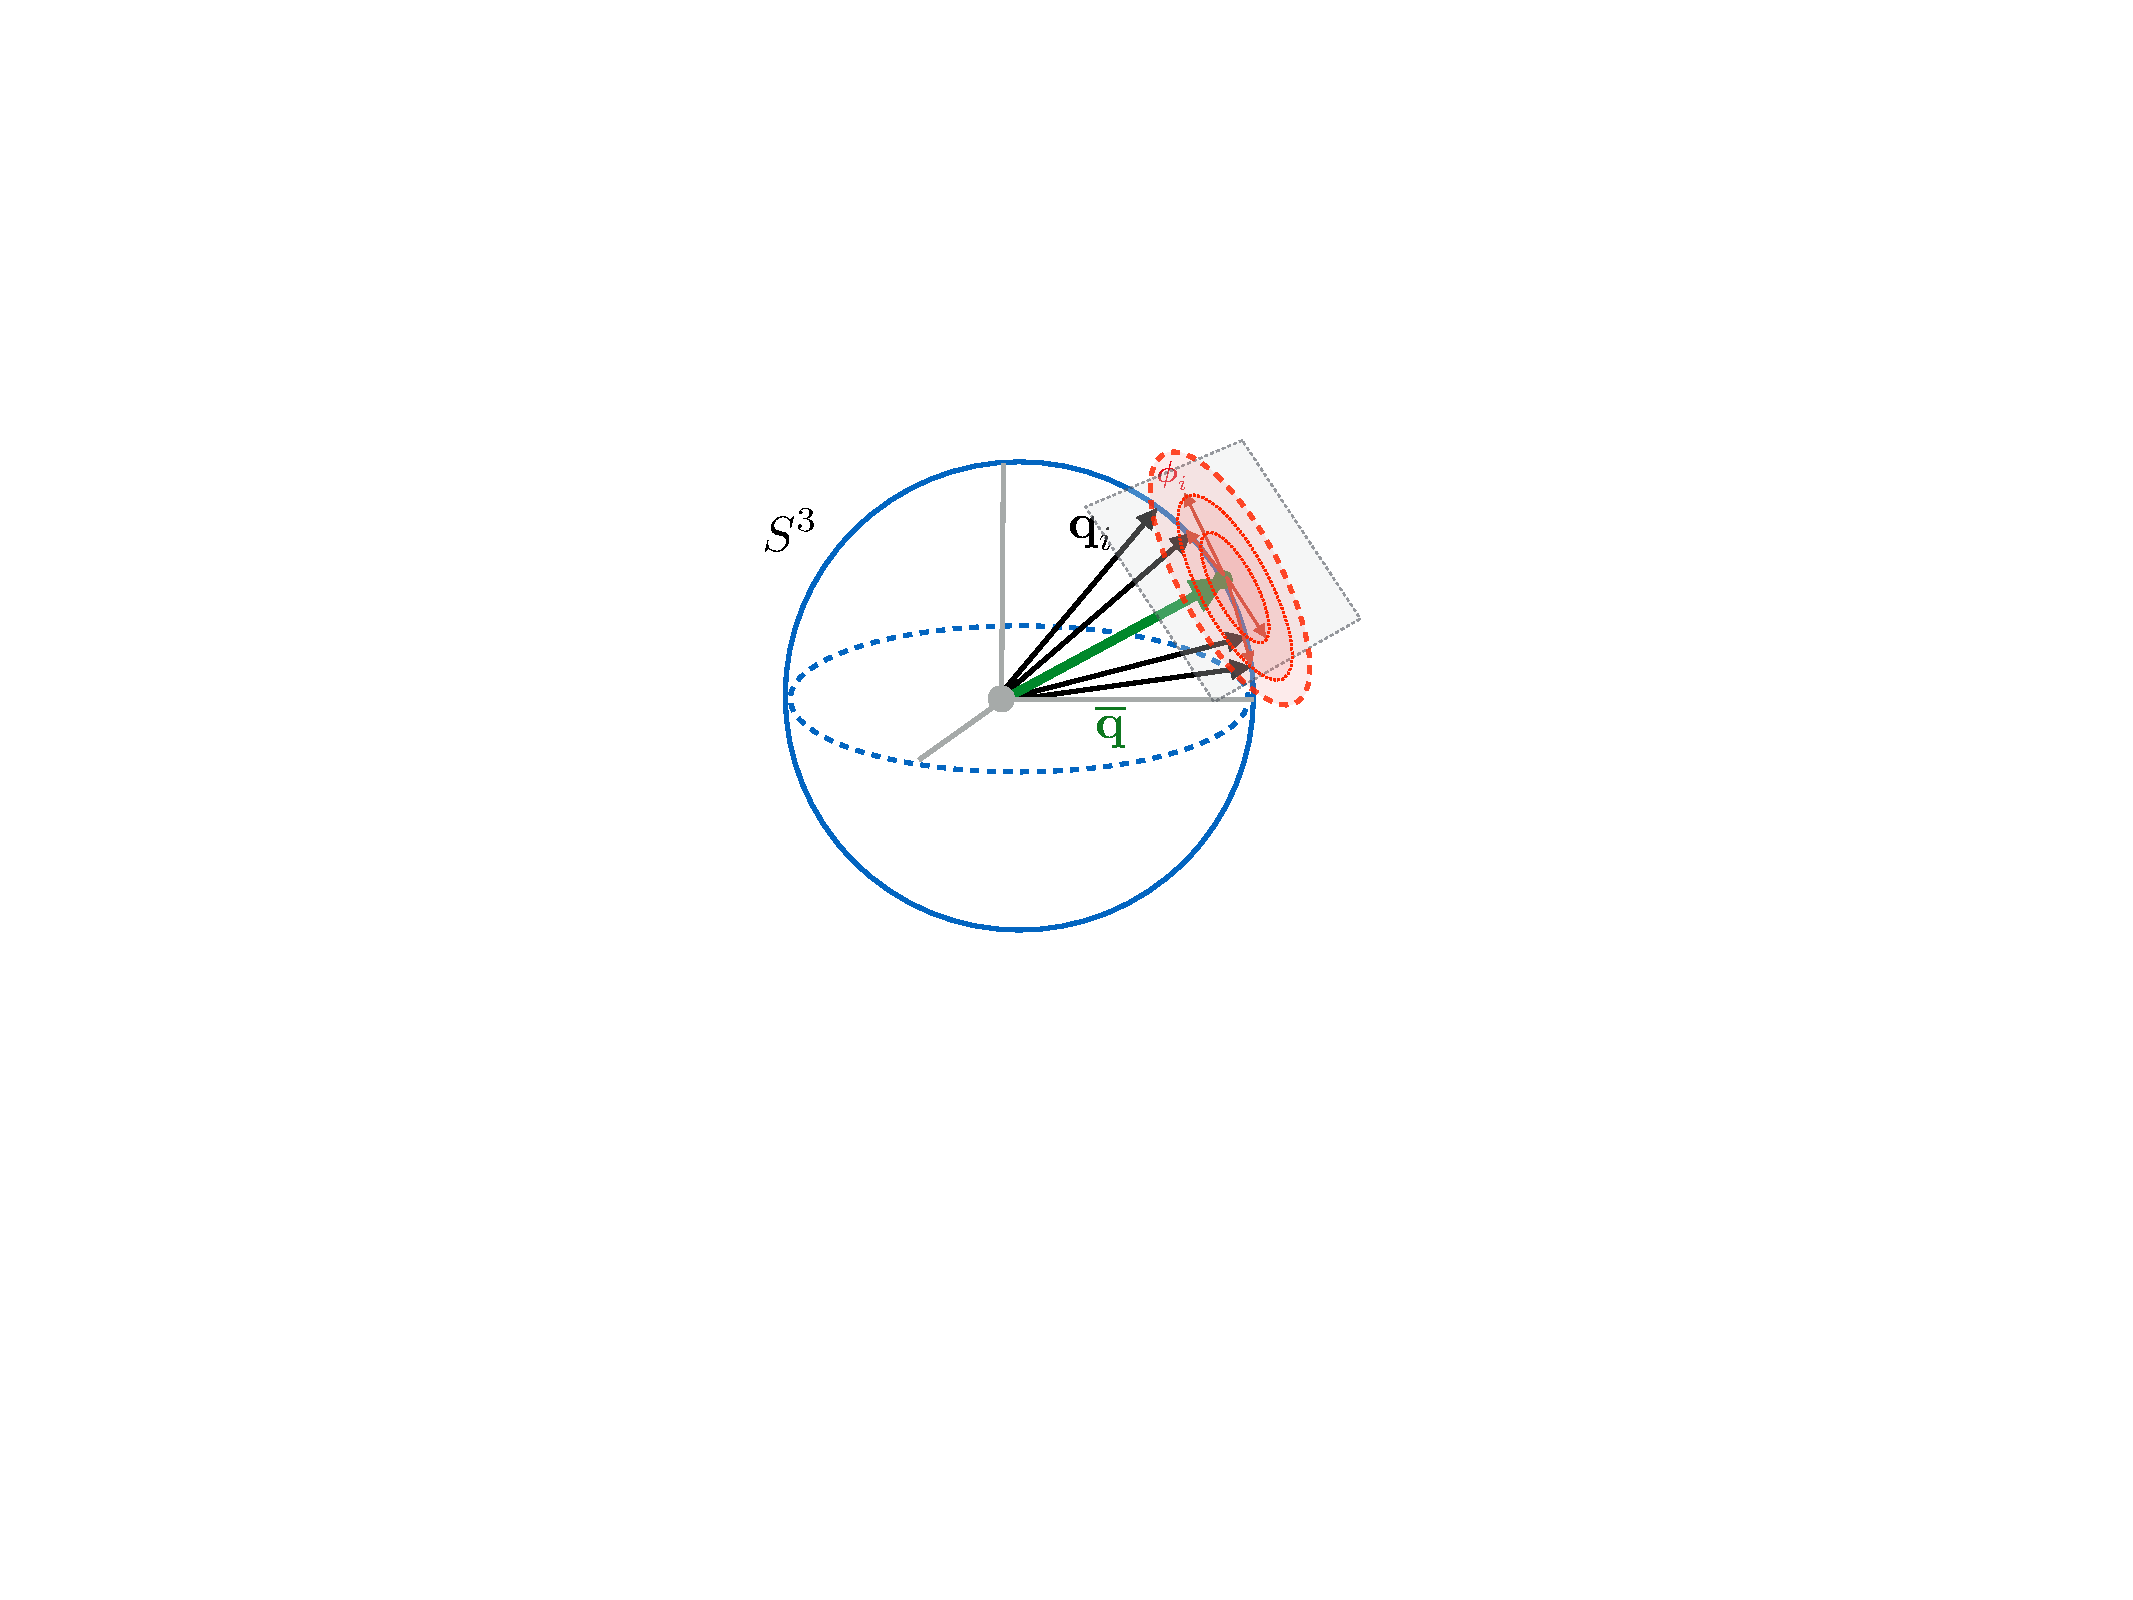
\includegraphics[width=0.33\textwidth]{math/quaternion_uncertainty.pdf}
  \end{center}
    \vspace{-20pt}
	\label{fig:math_quat_uncertainty}
	\caption{We can define uncertainty in the left tangent space of a mean element of a Lie group (here illustrated for unit quaternions).}
\end{wrapfigure} 


We can also use perturbation theory to implicitly define uncertainty on constrained manifolds (see \cite{Barfoot2014-ac} for a thorough discussion). 

Given a concentrated normal density, $\delta \TransformVector \sim \NormalDistribution{}(\Matrix{0}, \Matrix{\Sigma}_{6 \times 6})$, we can \textit{inject} this unconstrained density onto the Lie group through left perturbations about some mean using
\begin{align}
\Transform &= \MatExp{\delta \TransformVector} \Mean{\Transform}. 
\end{align}
This allows us to keep track of a random variable, $\Transform$, by keeping its mean in group form, $\Mean{\Transform}$, while its second statistical moment is stored as a standard $6 \times 6$ covariance matrix, $\Matrix{\Sigma}$.

We can define an analogous density for rotation matrices given normal densities over rotation perturbations $\delta \RotationVector \sim \NormalDistribution{}(\Matrix{0}, \Matrix{\Sigma}_{3 \times 3})$,
\begin{align}
\Rotation &= \MatExp{\delta \RotationVector} \Mean{\Rotation}, 
\end{align}
and also, for unit quaternions,
\begin{align}
\quat &= \MatExp{\delta \RotationVector} \otimes \Mean{\quat} 
\end{align}
where $\otimes$ refers to the standard quaternion product operator \cite{Sola2017quaternion}. %\todo{Add discussion of banana density this induces for SE(3) and the impossibility of known position but unknown rotation}.



 